\documentclass[parskip=full,11pt]{scrartcl}
\usepackage[utf8]{inputenc}
\usepackage[T1]{fontenc}
\usepackage[german]{babel}
\usepackage[useregional]{datetime2}
\usepackage[pdfborderstyle={/S/U/W 0}]{hyperref}
\usepackage[nameinlink]{cleveref}
\usepackage[section]{placeins}
\usepackage{xcolor}
\usepackage{graphicx}
\usepackage{csquotes}
\usepackage{amsmath} % for $\text{}$
\usepackage{pflichtenheft}

\newcommand\urlpart[2]{$\underbrace{\text{\texttt{#1}}}{\text{#2}}$}

\crefname{figure}{Abb}{Abb}

\hypersetup{
	pdftitle={Pflichtenheft},
	bookmarks=true,
}

% section numbers in margins:
\renewcommand\sectionlinesformat[4]{\makebox[0pt][r]{#3}#4}

% header & footer
\usepackage{scrlayer-scrpage}
\lofoot{\today}
\refoot{\today}
\pagestyle{scrheadings}

\newcommand\producttitle{GO-App}

\title{Pflichtenheft: \producttitle}
\author{Lukas Dippon
        \and Jens Kienle
        \and Matthias Noll
        \and Fabian Röpke
        \and Tim Schmidt
        \and Simon Vögele}

\begin{document}
\maketitle

\section{Einleitung}
Studenten und Mitarbeiter des KIT treffen sich gerne zum gemeinsamen Essen oder Lernen.
Dazu ist an einem bestimmten Tag immer notwendig zu wissen, ob bereits ein Treffen vereinbart wurde.
Am Treffpunkt angekommen, möchte man wissen, an welchem Ort sich die Gruppe befindet, um nicht lange suchen zu müssen.
Unsere App soll es angemeldeten Benutzern ermöglichen, sich in Gruppen zu organisieren.
In den Gruppen kann der Zeit- und Treffpunkt bestimmt werden.
Nach der Festlegung des Treffens soll die App die GPS-Standorte der Mitglieder temporär anzeigen, um das Treffen zu vereinfachen.

\pagebreak
%%%%%%%%%%%%%%
\section{Kriterien}
% Diese Section sollte kurz und knapp "für Manager" sein
% und auf eine Seite passen.

\subsection{Muss}
\criterium{Gruppen}{crt:groups}{10}
Mehrere Nutzer können sich in Gruppen zusammenschließen.
Ein Nutzer kann in beliebig vielen Gruppen Mitglied sein.

\criterium{Eigene Position auf Umgebungskarten}{crt:location}{20}
Der Nutzer ist in der Lage, seine aktuelle Position auf einer Karte der nahen
Umgebung einzusehen.

\criterium{Festlegbare Treffpunkte}{crt:meetingpoints}{30}
Innerhalb von Gruppen können Treffpunkte festgelegt werden,
die den Mitgliedern auf der Karte angezeigt werden.

\criterium{Gegenseitige Ortung}{crt:positions}{40}
Nutzer sind in der Lage, ihre aktuelle Position mit anderen Gruppenmitgliedern
über einen festlegbaren Zeitraum zu teilen.
Diese wird dann allen Gruppenmitgliedern auf der Karte angezeigt und laufend
aktualisiert.

\criterium{Datenschutz}{crt:privacy}{50}
Die Positionsdaten des Nutzers werden nur während des festgelegten Zeitraumes
(\criteriumlink{crt:positions}) gesendet und serverseitig nicht
längerfristig gespeichert.

\criterium{Nutzerkonten}{crt:account}{60}
Ein persönliches Nutzerkonto ermöglicht es Nutzern,
Gruppenzugehörigkeiten und Datenschutzoptionen zu speichern.

\subsection{Kann}
\criteriumOptional{Abstimmungen}{crt:vote}{10}
Innerhalb von Gruppen können die Nutzer über nächste Treffpunkte abstimmen.

\criteriumOptional{1 zu 1 Verbindung}{crt:1to1}{20}
Der Positionsaustausch zwischen zwei einzelnen Nutzern außerhalb von Gruppen
soll möglich und besonders einfach sein.
% TODO: „Besonders einfach“ zu schwammig?

\criteriumOptional{Detailliertere Innenraumkarten}{crt:indoor}{30}
Innenräume mit hoher Nutzerdichte bekommen detaillierte Innenraumkarten.

\criteriumOptional{Gruppenchat}{crt:chat}{40}
Innerhalb der Gruppen können simple Textnachrichten versendet werden.

\criteriumOptional{Eigene Server}{crt:ownServer}{50}
Es ist dem Nutzer möglich, einen eigenen Server zu erstellen und zu verwalten.

\criteriumOptional{Server-Wechsel}{crt:switchServer}{60}
Um \criteriumlink{crt:ownServer} ausnutzen zu können, ist es dem Nutzer
möglich, den verwendeten Server zu wechseln.

\criteriumOptional{Zeitplan für Positionsübertragung}{crt:timetable}{70}
Der Nutzer kann zu bestimmten Zeiten seine Position automatisch an bestimmte
Gruppen übertragen lassen.

\criteriumOptional{Passwortzurücksetzung}{crt:passwordReset}{80}
Der Nutzer kann sein Passwort zurücksetzen lassen, wenn er sich über eine zuvor
festgelegte E-Mail-Adresse authentifizieren kann.

\subsection{Abgrenzung}
\criteriumNot{Kein Social Network}{crt:socialNetwork}{10}
Die App bietet keine Plattform um Bilder oder andere persönliche Eindrücke mit
anderen zu teilen.

\criteriumNot{Kontakt nur zu Freunden}{crt:friendsOnly}{20}
Die App möchte die Kommunikation in bereits bestehenden Gruppen vereinfachen,
nicht den Kontakt zu Fremden ermöglichen.

\criteriumNot{Beidseitiges Einverständnis}{crt:consensual}{30}
Die Anwendung ermöglicht nicht das Orten von Personen,
die ihre Position nicht ausdrücklich zugänglich machen.
Beispielsweise können Eltern nicht ihre Kinder ständig mit dieser App orten.

\pagebreak
%%%%%%%%%%%%%%
\section{Produkteinsatz}
Das Produkt dient zur Erleichterung des Zusammenfindens und der
Treffpunktvereinbarung in geschlossenen Gruppen von Freunden, Kollegen oder
Familienmitgliedern.

\subsection{Anwendungsbereiche}
\begin{itemize}
    \item Private Treffen in der Freizeit oder während der Arbeit
    \item Zusammenfindung auf größeren Veranstaltungen
\end{itemize}

\subsection{Zielgruppen}
\begin{itemize}
    \item Freundesgruppen
    \item Arbeitskollegen
    \item Familien
\end{itemize}

\subsection{Betriebsbedingungen}
\begin{itemize}
    \item Mobiler Einsatz in Umgebungen mit GPS-Empfang und Zugang zum Internet
\end{itemize}

%%%%%%%%%%%%%%
\section{Produktumgebung}
Das Produkt beinhaltet ein Client-Server-Modell.
Der Server dient lediglich als Vermittler zwischen Klienten.
Die Nutzer verwenden den Klienten auf ihrem mobilen Endgerät.
\subsection{Software}
\begin{itemize}
    \item Client: Android 6 (\enquote{Marshmallow}, API-Level 23) oder
        höher.
    \item Server: Apache Tomcat 8
\end{itemize}

\subsection{Hardware}
% TODO: Mindestanforderungen an Hardware-Performance
\begin{itemize}
    \item Client: Android-fähiges mobiles Endgerät mit
        \begin{itemize}
            \item GPS-Empfänger
            \item Netzwerkkarte mit WLAN-Modul oder Mobilfunkeinheit
        \end{itemize}
    \item Server: Handelsüblicher Servercomputer, der Apache Tomcat 8
        unterstützt und eine Internetanbindung besitzt.
\end{itemize}

%%%%%%%%%%%
\section{Funktionale Anforderungen}

\subsection{Muss}

\functionality{Benutzerkonten}{fnc:account}{10}
\fulfills{crt:account}
Der Benutzer wird beim Starten der Anwendung aufgefordert, sich ein
Benutzerkonto zu erstellen oder sich mit einem bereits vorhandenen anzumelden.

\functionality{Gründen von Gruppen}{fnc:groupfounding}{30}
\fulfills{crt:groups}
Nutzer können Gruppen erstellen und diese verwalten, indem sie andere Nutzer
hinzufügen oder entfernen.

\functionality{Umgebungskarte}{fnc:map}{60}
\fulfills{crt:location}
Der Nutzer kann eine Karte aufrufen, auf dem seine eigene Position angezeigt
wird.

\functionality{Erstellung von Verabredungen innerhalb von Gruppen}
    {fnc:meetingpoints}{70}
\fulfills{crt:meetingpoints}
Der Nutzer kann innerhalb einer Gruppe eine Verabredung, bestehend aus einer
Zeit und einem Treffpunkt, erstellen, der allen Gruppenmitgliedern auf der
Umgebungskarte (\functionalitylink{fnc:map}) angezeigt wird.

\functionality{Übertragung der eigenen Position an die Gruppe}
    {fnc:positions}{90}
\fulfills{crt:positions}
Der Nutzer kann seine aktuelle Position an die Gruppenmitglieder übertragen.
Übertragene Positionen werden allen Gruppenmitgliedern auf der Umgebungskarte
(\functionalitylink{fnc:map}) angezeigt.
Steht eine Verabredung an, wird der Nutzer automatisch gebeten, seine Position
für die Dauer der Verabredung freizugeben.
Es ist ebenfalls möglich, andere Gruppenmitglieder zum Übertragen ihrer
Position aufzufordern.

\functionality{Verwaltung von Kontodaten}{fnc:options}{20}
\fulfills{crt:account}
Der Nutzer soll folgende Änderungen an seinem Konto vornehmen können:
\begin{itemize}
    \item Mit dem Konto verbundenes Passwort ändern
    \item Mit dem Konto verbundene E-Mail-Adresse ändern
    \item Konto löschen
\end{itemize}

\functionality{Verabredungsliste}{fnc:eventlist}{80}
\fulfills{crt:groups}
\fulfills{crt:meetingpoints}
Der Nutzer kann eine Liste aufrufen, in der alle Verabredungen aller Gruppen
des Nutzers nach Zeitpunkt sortiert angezeigt werden.

\subsection{Kann}

\functionality{Abstimmungen}{fnc:vote}{10}
\fulfills{crt:vote}
Der Nutzer kann innerhalb von Gruppen Abstimmungen erstellen.
Diese werden zeitlich begrenzt.
Der Abstimmung lassen sich beliebig viele Treff- und Zeitpunkte hinzufügen,
sowie Stimmen abgeben und verändern.
Alle zur Wahl stehenden Treffpunkte werden dabei als solche auf der
Umgebungskarte (\functionalitylink{fnc:map}) markiert.
Nach Ablauf des Zeitlimits wird jeweils eine Verabredung, bestehend aus dem
Treff- und Zeitpunkt mit den meisten Stimmen, erstellt.
Alle anderen Treff- und Zeitpunkte werden verworfen.

\functionality{Gruppenchat}{fnc:chat}{20}
\fulfills{crt:chat}
Jede Gruppe verfügt über einen Chat, in dem simple Nachrichten an alle
Gruppenmitglieder versandt werden können.

\functionality{Detaillierte Innenraumkarten}{fnc:indoor}{30}
\fulfills{crt:indoor}
Für Innenräume, in denen eine hohe Nutzerdichte erwartet wird, werden
detaillierte Innenraumkarten in die Umgebungskarte integriert. Die Menge an
Innenraumkarten kann mit weiteren späteren Versionen noch erweitert werden.

\functionality{Eigene Server}{fnc:ownServer}{40}
\fulfills{crt:ownServer}
Es soll möglich sein, einen eigenen Server einrichten und diesen statt des
standardmäßig zur Verfügung stehenden Servers zu verwenden.
Zwischen verschiedenen Servern findet keine Kommunikation statt.
Insbesondere werden Nutzerkonten nur serverweit gespeichert.
Für die Einrichtung eines eigenen Servers wird keine Hardware zur Verfügung
gestellt und die benötigten Systemadministrationskenntnisse vorrausgesetzt.

\functionality{Serverwechel}{fnc:switchServer}{50}
\fulfills{crt:switchServer}
Das Wechseln des Servers soll innerhalb der App und noch vor dem Login in ein
Benutzerkonto möglich sein.

\functionality{Stummschalten}{fnc:mute}{60}
\fulfills{crt:groups}
Sowohl der Gruppenchat (\functionalitylink{fnc:chat}), als auch die
Abstimmungen (\functionalitylink{fnc:vote}) und Übertragungsanfragen
(\functionalitylink{fnc:positions}) lassen sich unabhängig voneinander
\enquote{stumm schalten}, d.h. es lassen sich jegliche Benachrichtungen für den
Nutzer unterdrücken.

\functionality{Zeitplan für Positionsübertragung}{fnc:timetable}{70}
\fulfills{crt:timetable}
Der Nutzer kann einzelnen Gruppen einen persönlichen wöchentlichen Zeitplan
zuteilen, in dem er festlegt, zu welchen Zeiten er automatisch seine Position
in der Gruppe freigibt.

\functionality{Passwortzurücksetzung}{fnc:passwordReset}{60}
\fulfills{crt:passwordReset}
Hat ein Nutzer sein Passwort vergessen, kann er eine E-Mail an seine zuvor
mit dem Konto verbundene E-Mail-Adresse senden lassen.
In dieser E-Mail sind Zugangsdaten, mit denen er sich temporär auch ohne das
Passwort authentifizieren und das Passwort ändern kann.
Dabei wird das vorherige Passwort nicht preisgegeben.

%%%%%%%%%%

\section{Nicht-Funktionale Anforderungen}

\nonFunctionality{Standortteilung für zwei einzelne Personen}{nfc:1to1}{10}
\fulfills{crt:1to1}
Es soll für zwei Einzelpersonen noch einfacher sein, ihren Standort miteinander
zu teilen. Dies soll in wenigeren Schritten möglich sein, als manuell eine
Gruppe aus zwei Leuten zu erstellen.

\nonFunctionality{Einfache Bedienung}{nfc:handling}{20}
Damit die App sich gegen die gängigen Instant Messenger durchsetzen kann, muss
sie intuitiv und einfach bedienbar sein. Um dies zu erreichen, erfüllt die
graphische Benutzeroberfläche die \enquote{Material Design}-Richtlinien.

\nonFunctionality{Ressourcennutzung}{nfc:resourceUsage}{30}
Um Akkulaufzeit und mobiles Datenvolumen zu sparen, findet die Aktualisierung
von Positionsdaten maximal einmal pro Sekunde statt.

\nonFunctionality{Mobile Nutzung}{nfc:connectionLoss}{40}
Verbindungsabbrüche, wie sie im mobilen Netz öfter auftreten, führen nicht zu
Fehlfunktionen.

\nonFunctionality{Nutzeraufkommen}{nfc:userLoad}{50}
Es müssen mindestens 1000 Nutzer die Anwendung in Verbindung mit dem gleichen
Server gleichzeitig verwenden können.

\nonFunctionality{Datenschutz}{nfc:privacy}{60}
Der Umgang mit Nutzerdaten entpricht den national geltenden
Datenschutzgesetzen.

\nonFunctionality{Datenspeicherung}{nfc:data storage}{70}
Daten über Standorte werden serverseitig nur so lange gespeichert, wie diese
für andere Nutzer einsehbar sein sollen.

%%%%%%%%%%%
\section{Tests}

\test{Gruppe Erstellen}{tst:grpcreate}{10}
\tests{fnc:account}

\teststep{Nutzer \enquote{Ned Stark} ist eingeloggt.}
{Ned tippt auf den Tab  \enquote{Gruppen}.}
{Er bekommt die Liste aller Gruppen angezeigt in denen er Mitglied ist.}

\teststep{Ned möchte eine Gruppe mit Leuten aus dem Fußball-Training erstellen.}
{Er tippt auf den \enquote{+}-Button (Neue Gruppe erstellen).}
{Er bekommt eine Liste all seiner Kontakte, die er im Produkt hinzugefügt hat, angezeigt.}

\teststep{Seine Freunde Robert B. und Edmund T. spielen ebenfalls Fußball.}
{Er tippt die beiden Namen an.}
{Das Produkt schlägt ihm vor die Gruppe zu erstellen.}

\teststep{Ned hat keine weiteren Freunde.}
{Er tippt auf Gruppe erstellen}
{Der Homescreen der Gruppe wird angezeigt.} % TODO: Homescreen?

%%%%%%%%%%%%%
\pagebreak
\appendix

\section{Seitenentwürfe}

% made via https://gomockingbird.com/projects/mnf0cwf/4gXVnC

\begin{figure}[hb]
	\fbox{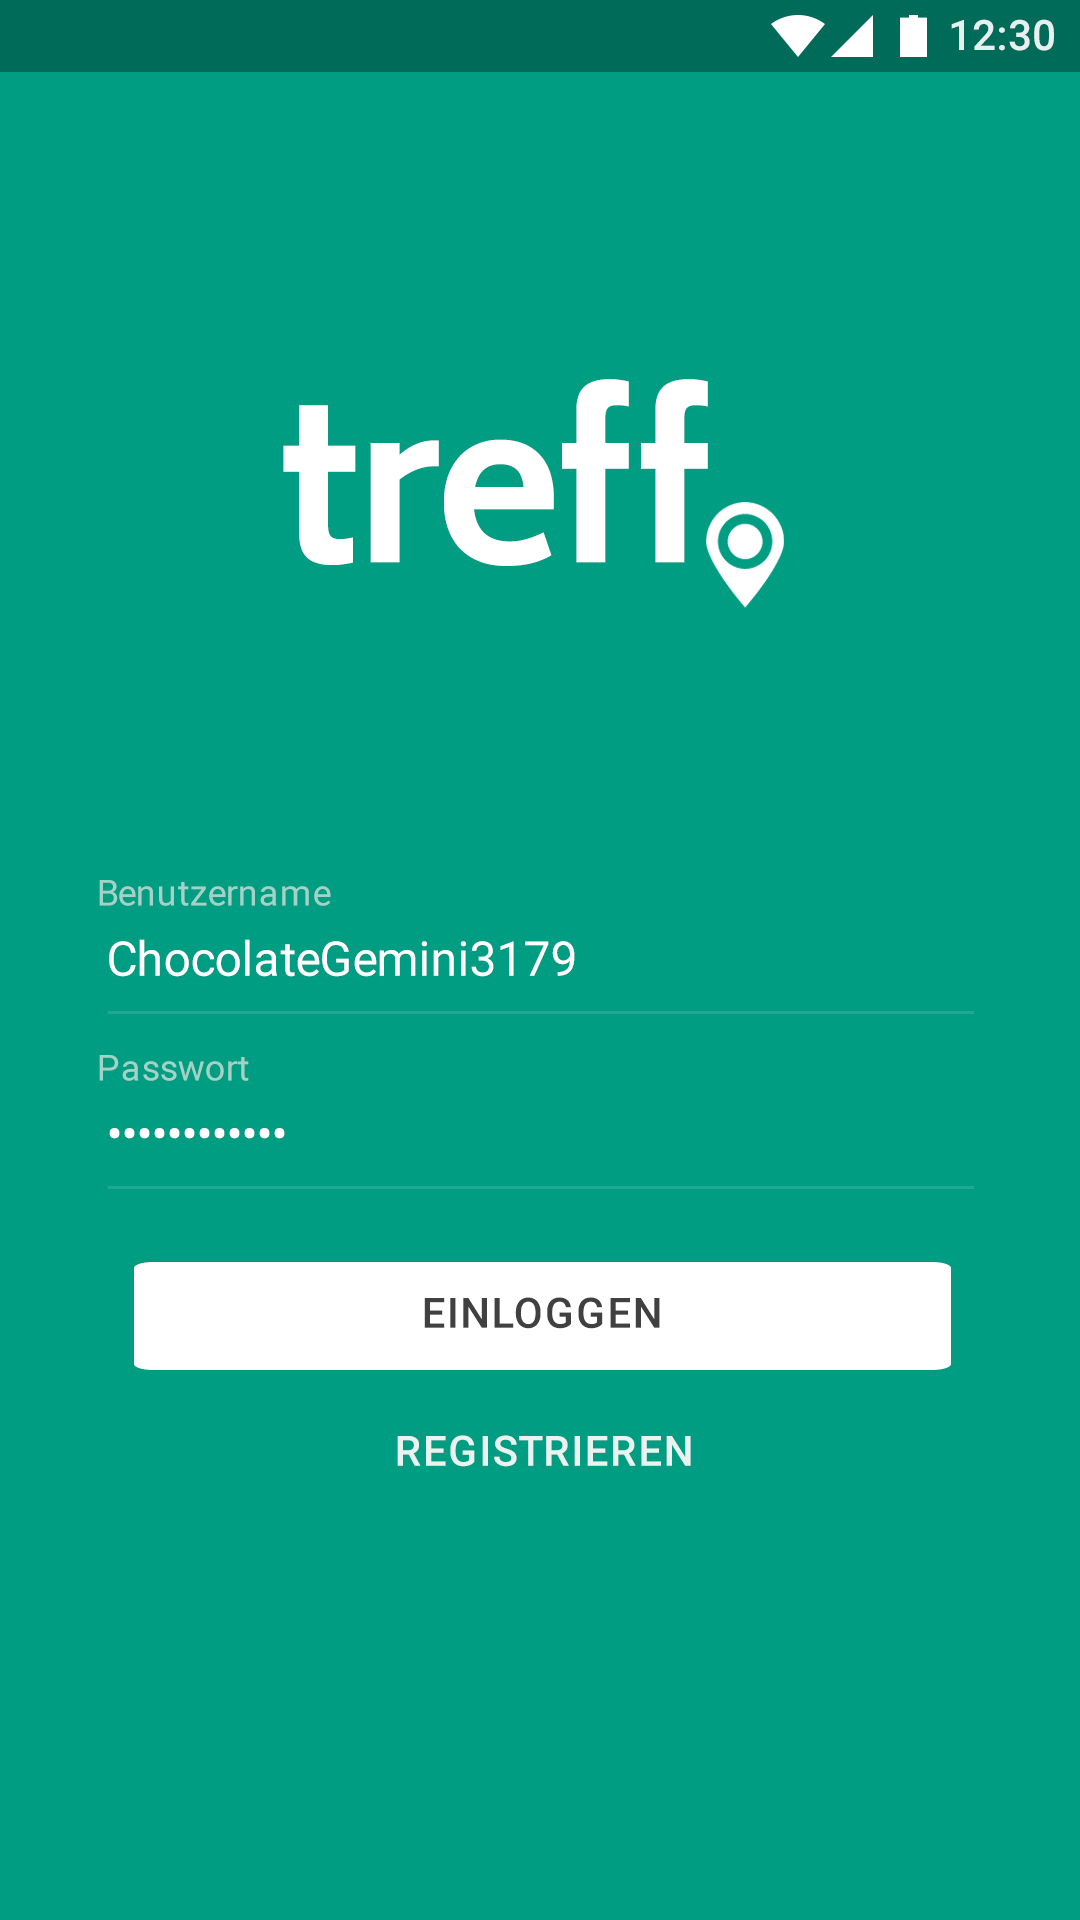
\includegraphics[height=80mm]{mockups/login.png}}
	\caption{\label{fig:menu}
		Login-Screen beim ersten Öffnen der App.
		 \testlink{tst:grpcreate}.
	}
\end{figure}

\begin{figure}[hb]
	\fbox{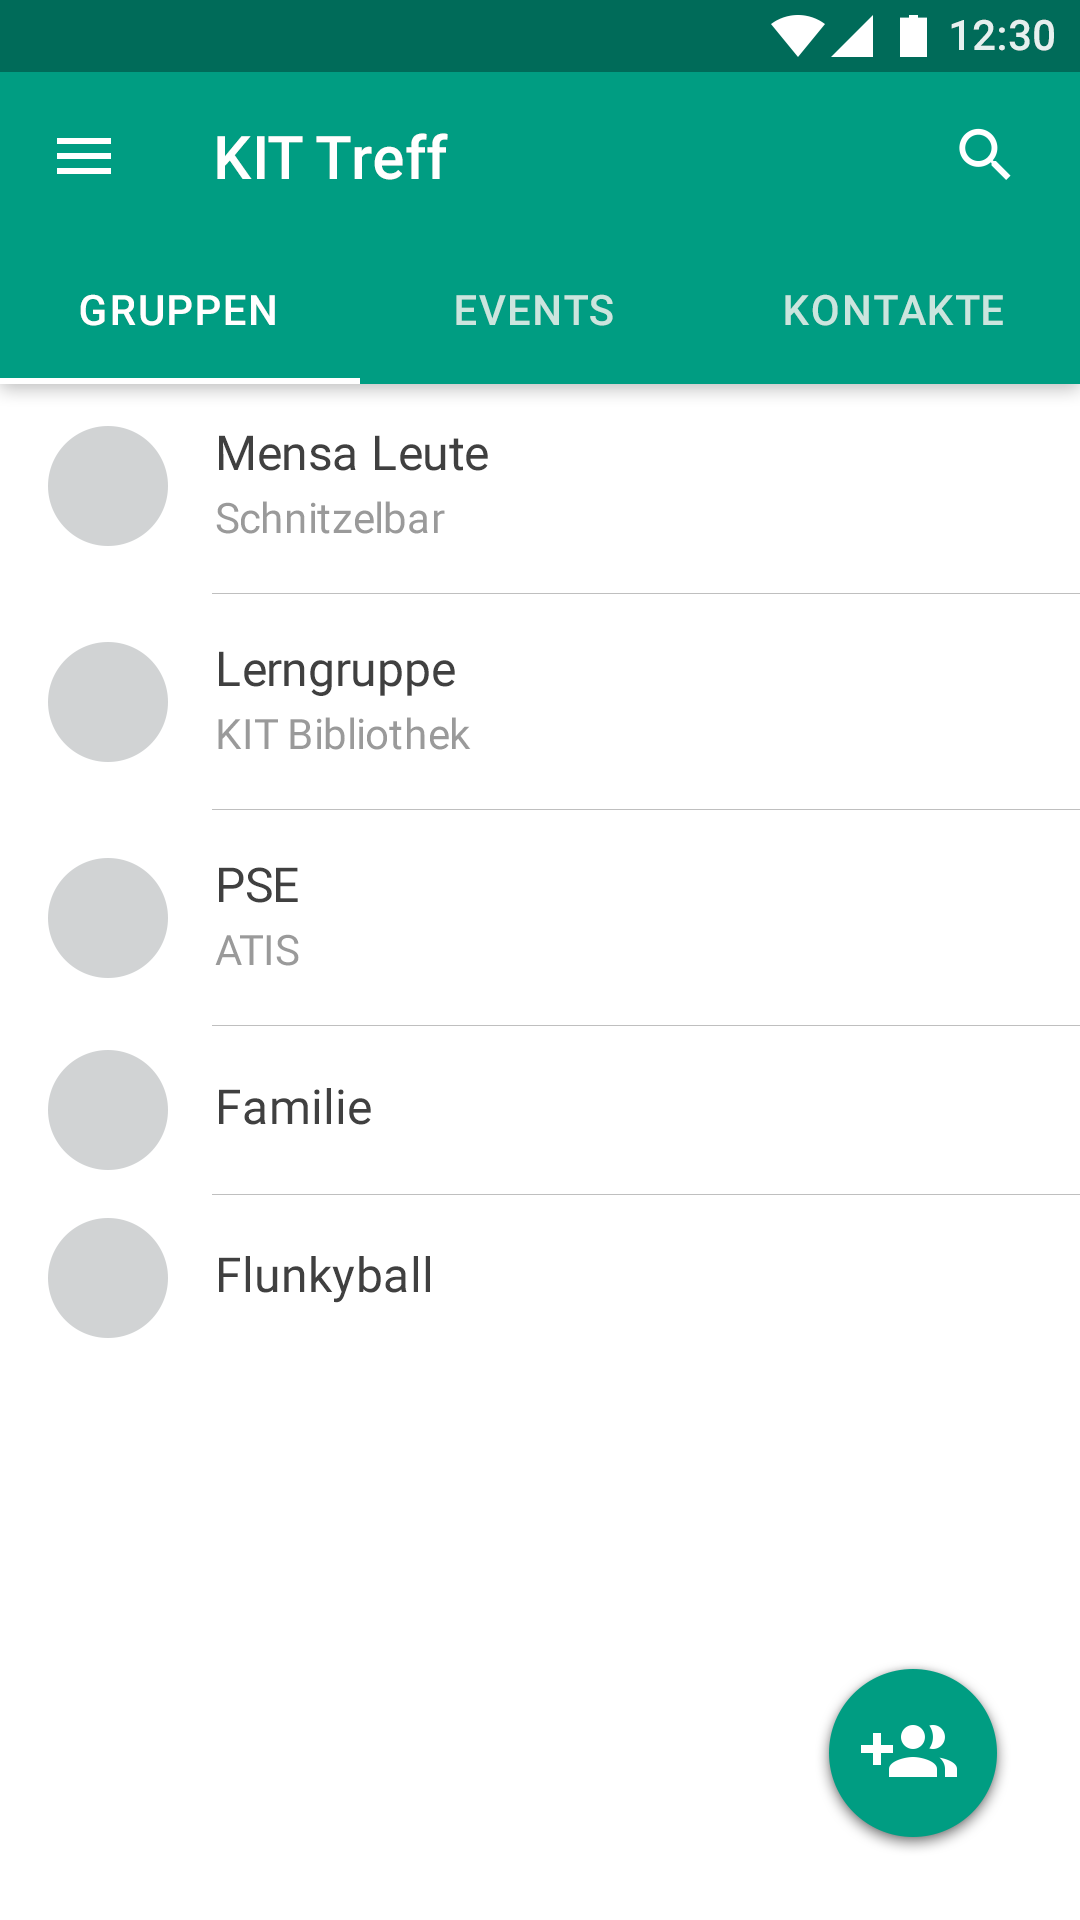
\includegraphics[height=80mm]{mockups/home_groups.png}}
	\caption{\label{fig:groups}
		Hier können Gruppen verwaltet und angesehen, sowie neue hinzugefügt werden.
		\testlink{tst:grpcreate}.
	}
\end{figure}

\begin{figure}[hb]
		\fbox{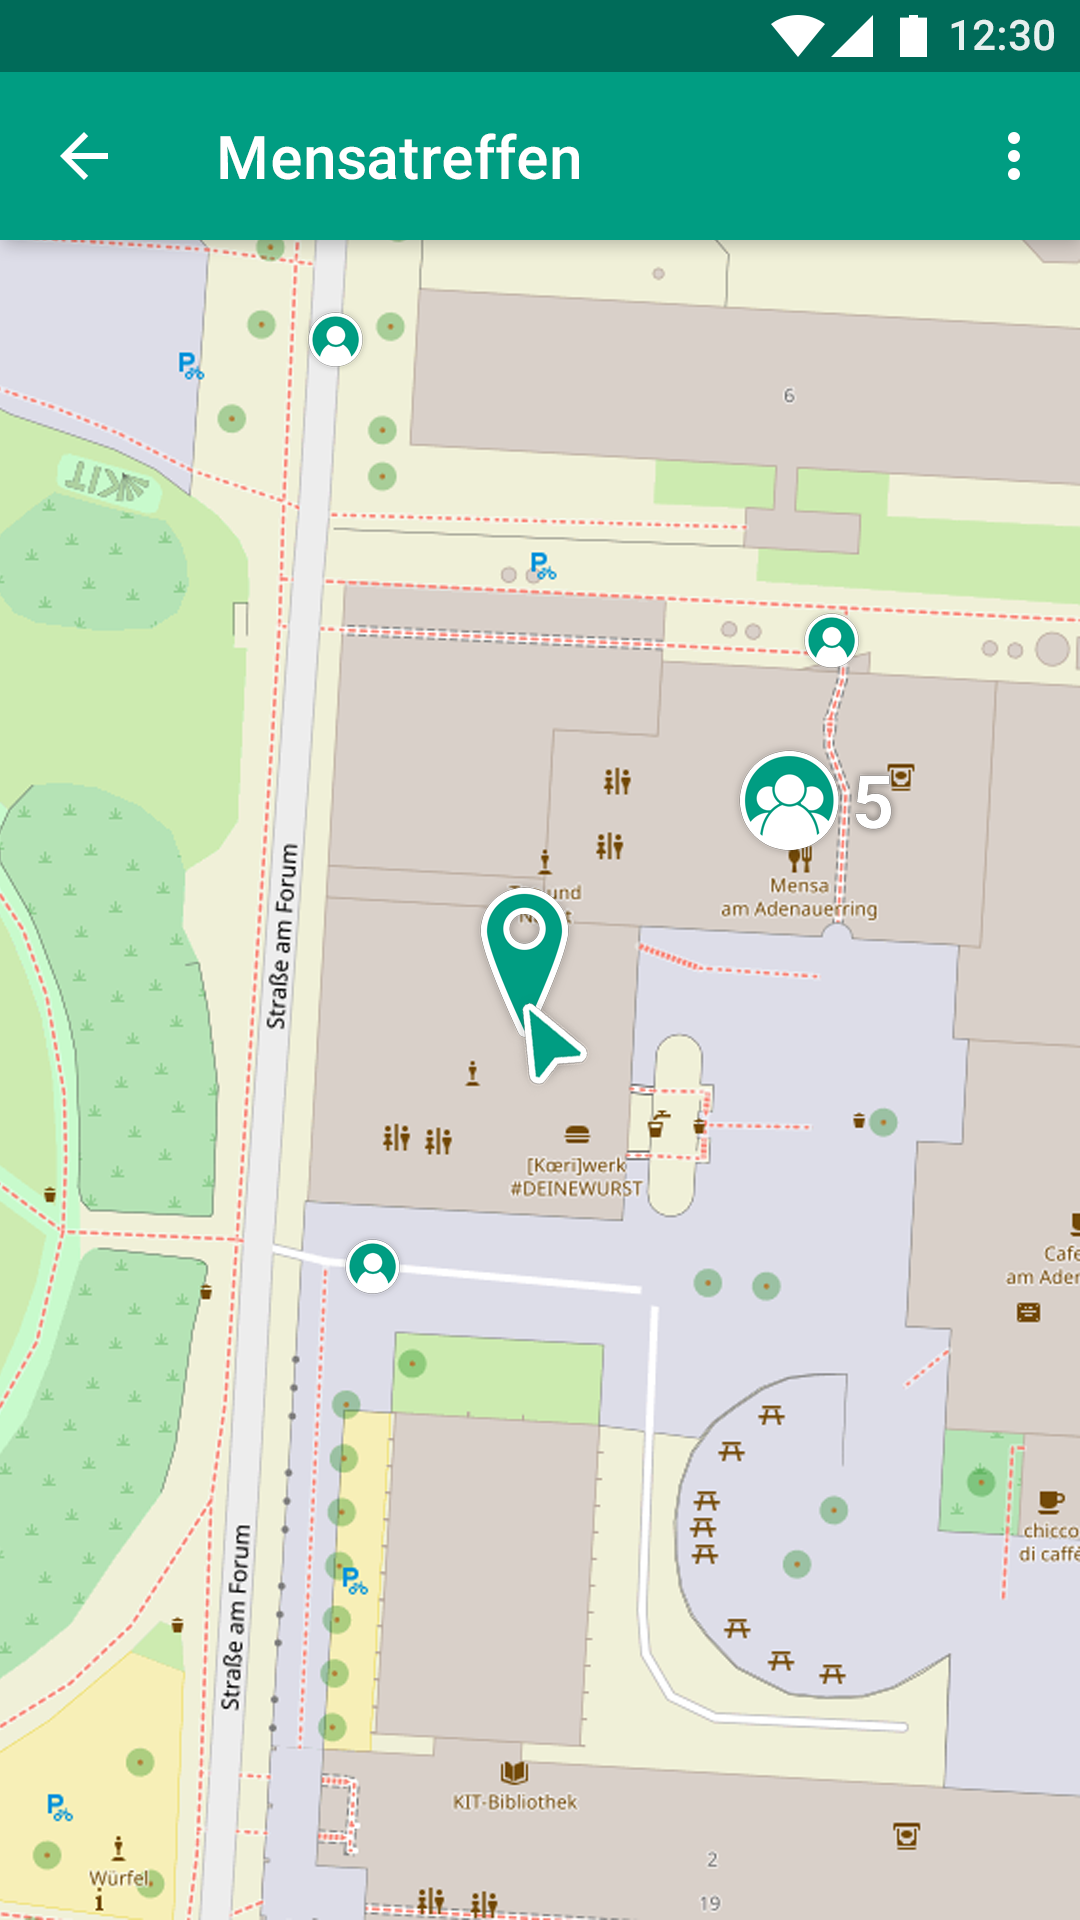
\includegraphics[height=80mm]{mockups/event_map.png}}
		\caption{\label{fig:map}
			Auf der Karte kann die Position der anderen Gruppenmitglieder eingesehen werden.
			Orte mit mehreren Mitgliedern erscheinen größer.
			\testlink{tst:grpcreate}.
		}
\end{figure}

\section{Glossar}

\textbf{Besucher}:
Eine Person, welche den Dienst nutzt.
Kann eingeloggt sein oder nicht.

\textbf{Nutzer}:
Ein eingeloggter Besucher.

\textbf{Gruppe}:
Mehrere Nutzer, welche untereinander Positionsdaten austauschen können.

\textbf{Chat}:
Möglichkeit für Mitglieder einer Gruppe, Textnachrichten auszutauschen.

\end{document}
